
To cross-validate the robustness of the initials results, I re-estimate the models with altered methods in order to confirm that the appearance of over-performance is not created artificially. Thus, the practice can lead to validation or invalidation of the methodologies. On top if this, it can further increase our understanding of the underlying drivers of shareholder behavior. \\
I make two adjustments for the Market Model and the Calendar-Time Portfolio. First, the threshold for events to be considered as important is modified to two and three standard deviations. Second, I change the portfolio weight from being determined by market capitalization (value weights) to a naive approach (equal weights). Finally, I round off the chapter with an introduction to the relation between negative events and investor reactions on global companies. 

As the relation between positive events and returns appears to be insignificant and vague, which is also reflected in the re-estimated results, this section will focus solely on the relation to negative news. If needed, the graphs depicting reactions to positive events can be found in Appendix \ref{app: sensitivity}.

\subsection{Event Threshold} \label{sec: sens_st_sd}

The thresholds for event identification is primarily driven by the average volume of daily or monthly news articles for a specific firm over the entire sample period. Raising the threshold naturally leads to fewer stocks being included in the portfolio. Intuitively, tightening the threshold is anticipated to capture more extreme events, which is expected to result in higher abnormal returns. In other words, the stricter threshold focuses on capturing events that have a greater potential to generate substantial market reactions, potentially resulting in more pronounced abnormal returns, if the causality holds true. 

\begin{figure} [H]
    \centering
    \caption{Threshold Value: Negative news}
    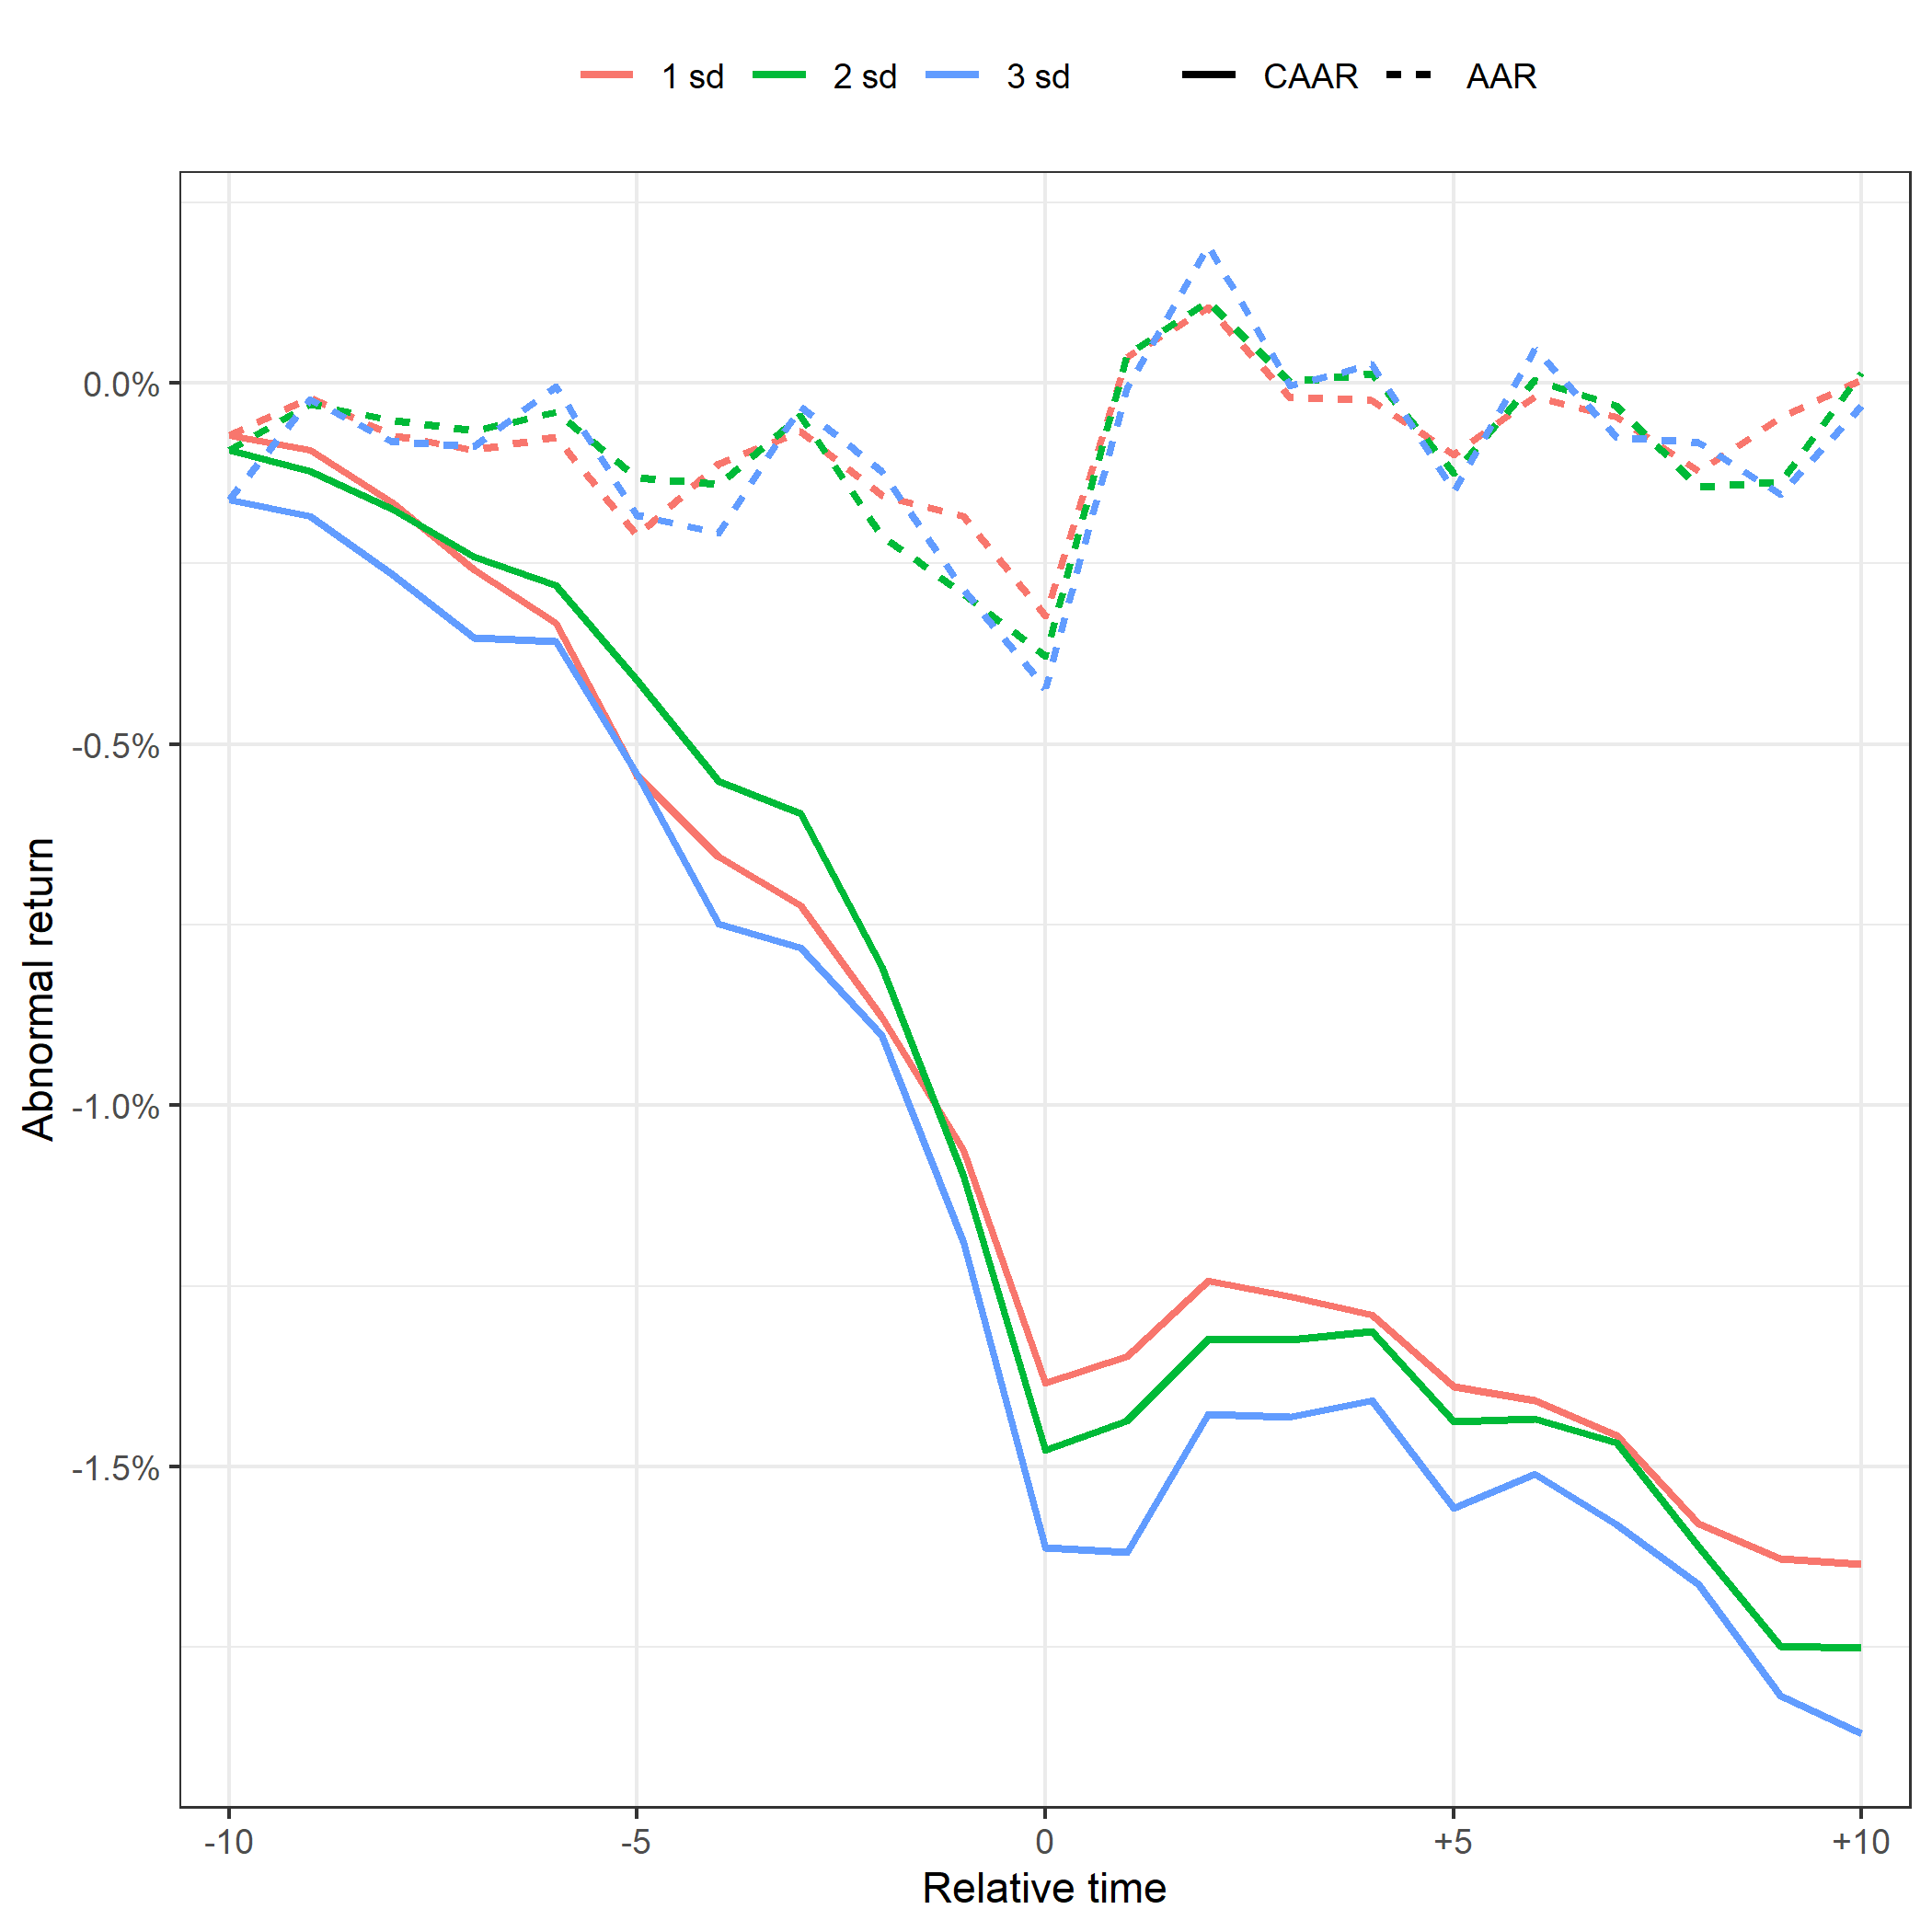
\includegraphics[scale=0.6]{Projekt/1.Figures analysis/ST_negative_sensitivity.png}
     \caption*{\footnotesize The figure illustrates the AAR and CAAR around the event date (t = 0) of negative news. The various colors represent the event identification rule of 1, 2, or 3 standard errors. The groups have, respectively, 1618, 1,231, and 997 events for 1,2, and 3 standard deviations}
    \label{fig:ST_neg_sensitivity}
\end{figure} 

\textbf{Short term.} Figure \ref{fig:ST_neg_sensitivity} compares the outcomes from changing the threshold of events. The AAR is presented in dotted lines and the CAAR in solid lines for thresholds applying one standard deviation as originally (red), two standard deviations (green), and 3 standard deviations (blue). For simplicity, I omit the confidence intervals along with the bars. The similarity of the AARs and CAARs imply that the results are robust to changes in the methodology. 

Enforcing a tighter threshold leads to a greater immediate impact on the event date, indicated by the lower AAR on $t=0$ for both two and three standard deviation thresholds. However, the cumulative investor reaction over the entire window is less significant for the two and three standard deviation thresholds compared to one standard deviation. Thus, in contrast with common intuition, more extreme events leads to lower abnormal returns. At least from this methodology. 

\noindent \textbf{Long term.} Altering the threshold requirements from one to two and three standard leads to varying outcomes on the long horizon. When considering holding periods of one month, the alphas decrease and become statistically insignificant. The portfolio constructed using a threshold of three standard deviations produce larger alphas compared to the one with a threshold of two standard errors, with values of -0.78\% and -0.47\%, respectively. However, for a holding period of T = 4, the relation is reversed, with values of -0.27\% and -0.45\% respectively. For longer holding periods, the abnormal returns converge to approximately zero across different threshold values. As the portfolios are generating seemingly random, or at least fluctuating, outcomes, I reason that there is no relation between the event threshold and portfolio return on the long horizon, which aligns with the outcomes from the short term sensitivity control. However, although insignificant, the results support the relation between negative events and abnormal returns.  


 
\subsection{Portfolio Weights} \label{sec: sens_st_weights}

\textbf{Short term.} Figure \ref{fig:ST_neg_sensitivity_weight} compares the performance of applying value and equal weights to the portfolio. Both portfolios consist of the same sample of firms that have encountered a negative event. 

\begin{figure}[h]
    \centering
    \caption{Value vs. equal weights: Negative news }
    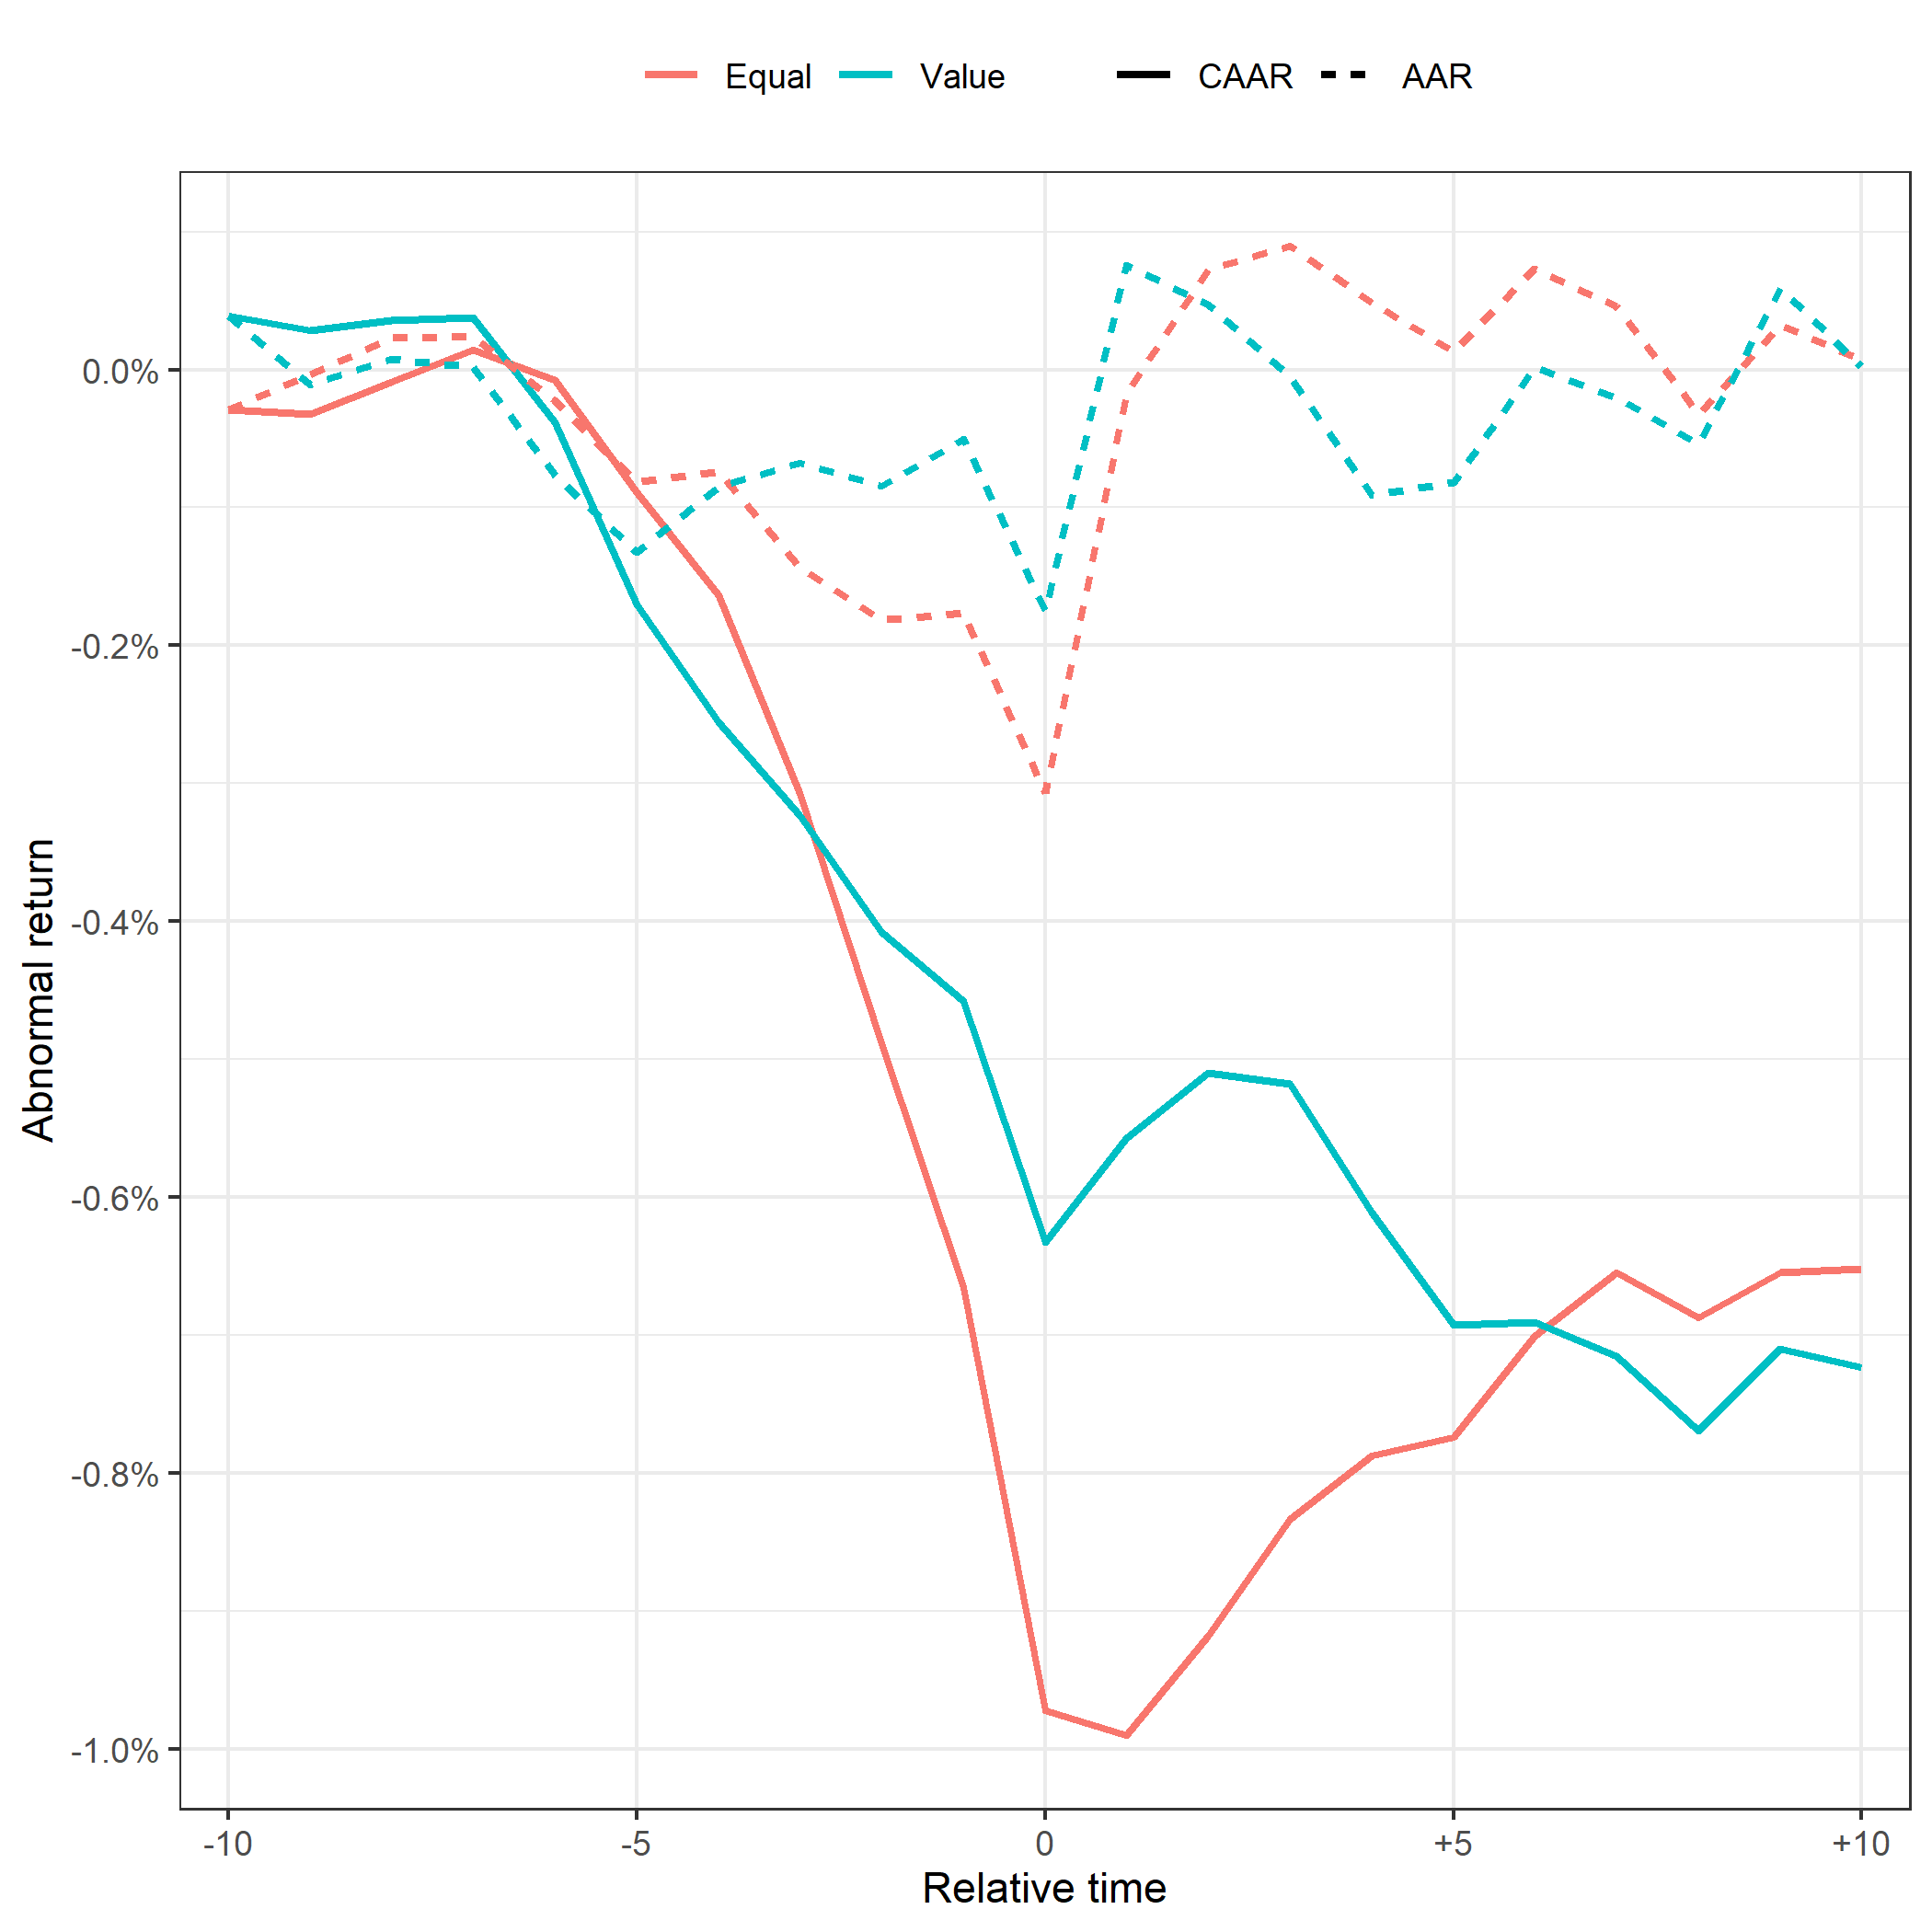
\includegraphics[scale=0.6]{Projekt/1.Figures analysis/ST_negative_sensitivity_weight.png}
     \caption*{\footnotesize The figure illustrates the average abnormal return (AAR) and cumulative AAR (CAAR) around the event date (t = 0) of negative news. The blue lines are returns calculated from an equally weighted portfolio, while the red lines are based on market capitalization weights.}
    \label{fig:ST_neg_sensitivity_weight}
\end{figure} 

From a visual perspective, the abnormal returns obtained by applying equal weights to the portfolio validate the original results, as the CAAR over the entire window is approximately equivalent to that of applying value weights. Although the portfolio AARs show a degree of similarity, the development of the CAAR is more adverse when applying equal weights compared to value weights. 

Applying equal weights to the portfolio inherently allocates more weight to smaller stocks, which contribute to a more severe initial investor reaction. In the days leading up to the event, the CAAR of the equal weighted portfolio declines at a faster rate compared to the value weighted portfolio, which results in a lower bottom of approximately 1.0\%. However, after the spike in negative news has occurred, the CAAR reverts to the same level as the value weighted portfolio. The observed pattern suggests that there is an initial overreaction among investors in the case of smaller stocks. As more information becomes available and the true magnitude of the event is revealed, the market adjusts its expectations and reevaluates the impact, ultimately bringing the performance of the portfolio in line with the value weighted portfolio.

\textbf{Long term.} Table \ref{tab: FF5_sensitivity} reports the alphas, t-values and significance levels of equally weighted portfolios, along with the results obtained by altering the threshold requirements. Besides the weights and thresholds, the portfolio construction is identical to that from the empirical results relating to negative events in section \ref{sec: long_term_portfolio}.   

Applying equal portfolio weights clearly indicate a discrepancy in the significance of the alphas compared to value weights. The equal weighted portfolio generates significant alpha values in all holding periods. Most notably, the equal weighted portfolio demonstrates significant alpha values of -0.64\% and -0.49\% with holding periods of eight and 12 months, respectively. In contrast, the value weighted portfolios yield insignificant alpha values of less than 0.05\% with the same holding periods. 

Across all holding periods, the results show a slight contrast with the short-term equal weighted portfolio, where the portfolio constructions generated approximately even abnormal returns over the full window. However, the short-term behavior displayed increased volatility and a lower minimum level of the CAAR when applying equal weights, aligning with the long term results. 
Moreover, the significant alpha values obtained when using holding periods of T = 8 and 12 months suggest that smaller stocks are penalized over a longer time horizon than relatively larger ones. 
Overall, the abnormal returns of the equal weighted portfolios confirm the negative association between negative events and abnormal returns on a short to medium time horizon. 

\setlength{\tabcolsep}{15pt}
\begin{table}[H]
\small
\centering
\caption{FF-5 alpha: Equal weights and threshold value } 
\makebox[\textwidth][c] {
\begin{tabular}{ccccccc}
\hline \hline \\ 
& &  Equal & & \multicolumn{2}{c}{ Value  } & \\ \cline{3-3} \cline{5-6}
  & & (1 SD) & & 2 SD  &  3 SD  & \\   
 & & & T = 1  & & \\ \cline{2-6}
 &  Alpha & $-0.96^{***}$  & &  -0.47  & -0.78  &  \\ 
 & t-value &  -3.80 &  & -0.97  & -1.63 & \\
 & &   & T = 4  & \\ \cline{2-6}
 & Alpha & $-0.70^{***}$ &  & $-0.45$ &  -0.27 & \\
 & t-value & -3.93 & & -1.58  & -1.04  & \\
 & &  & T = 8  & \\ \cline{2-6}
 & Alpha  & $-0.64^{***}$ & & -0.14 & -0.12 &  \\
 & t-value  & -4.20 & & -0.89 & -0.68 & \\
& &  & T = 12  & \\ \cline{2-6}
 & Alpha  & $-0.49^{***}$ &  & -0.16 & -0.17 &  \\
 & t-value & -3.71 & & -1.16 &  -0.97  & \\ \hline \hline
 \multicolumn{7}{l}{ \footnotesize $^* \; p\; <\; 0.1$, $ ^{**} \; p\; <\; 0.05$, $ ^{***} \; p\; <\; 0.01$  } \\
 \multicolumn{7}{p{12cm}}{ \footnotesize Alpha is the WLS-regression intercept (in \%) of the Fama-French 5-factor model, displayed along with the corresponding t-value. N is the average amount of firms included in the portfolio each month, and T is the portfolio holding period. The threshold for event firms to be included in the portfolio is either 1,2 or 3 "SD" (standard deviations) larger than the mean.} \\ 
 \hline
\end{tabular}
}
\label{tab: FF5_sensitivity}
\end{table}

\subsection{Inference from Global Companies}

To further assess the robustness of the main results, I reiterate the empirical analysis with a novel sample of firms and corresponding SDG news from the constituents of the Nasdaq Global Large Cap Index\footnote{https://indexes.nasdaqomx.com/Index/Overview/NQGLCI}. 

The inclusion of the new sample of firms offer valuable insights into the global perspective on the relationship between ESG factors and corporate performance. The abnormal returns on both short- and long-term returns has been through the same transformation as the ones from the original models. The Market Model applies the MSCI World Index\footnote{https://www.msci.com/World} as the market portfolio in the regressions, while the Calendar-Time Portfolio approach applies the Fama-French Developed Markets 5 factors\footnote{https://mba.tuck.dartmouth.edu/pages/faculty/ken.french/data$\_$Library/f-f$\_$5developed.html} in the regressions. 

\begin{figure} [H]
     \centering
     \begin{minipage}[b]{0.49\textwidth}
         \centering
    \caption{Global: Negative news}
    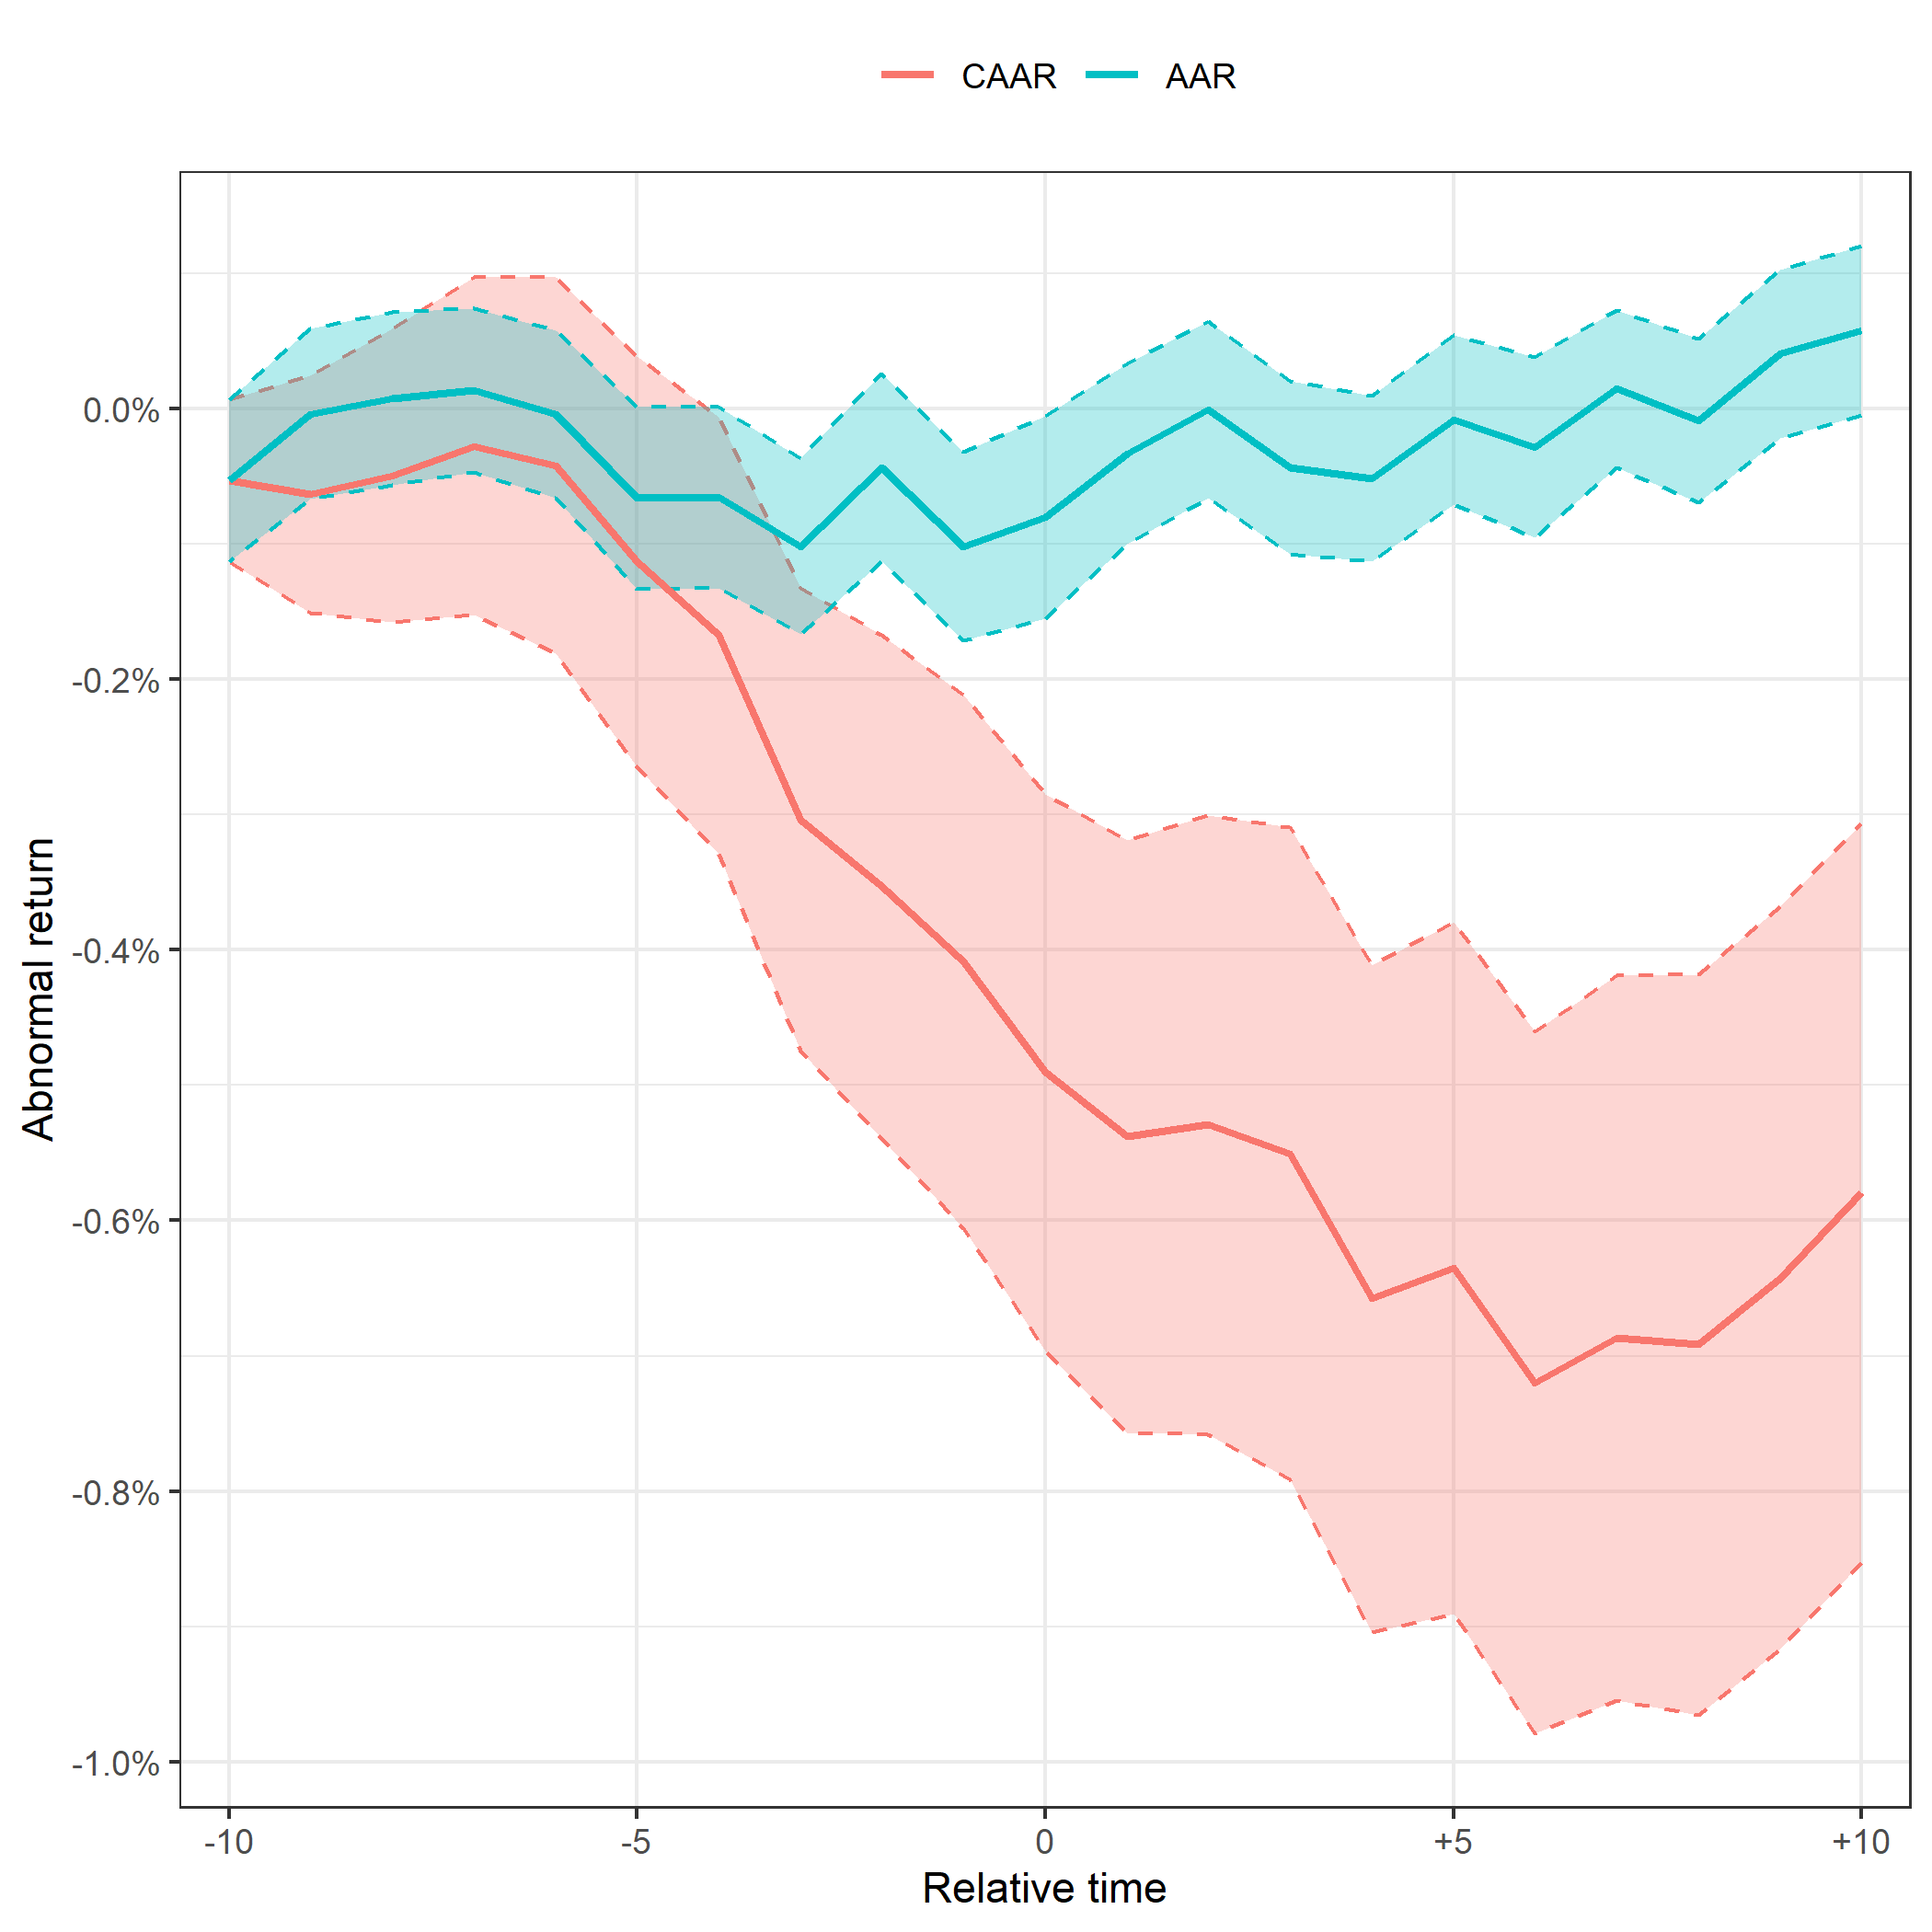
\includegraphics[width=\textwidth]{Projekt/1.Figures analysis/ST_negative_all_CI_nasdaq.png}
     \label{fig:ST_neg_sensitivity_nasdaq}
     \end{minipage}
     \hfill
     \begin{minipage}[b]{0.49\textwidth}
       \centering
    \caption{Global: Negative news, ESG}
    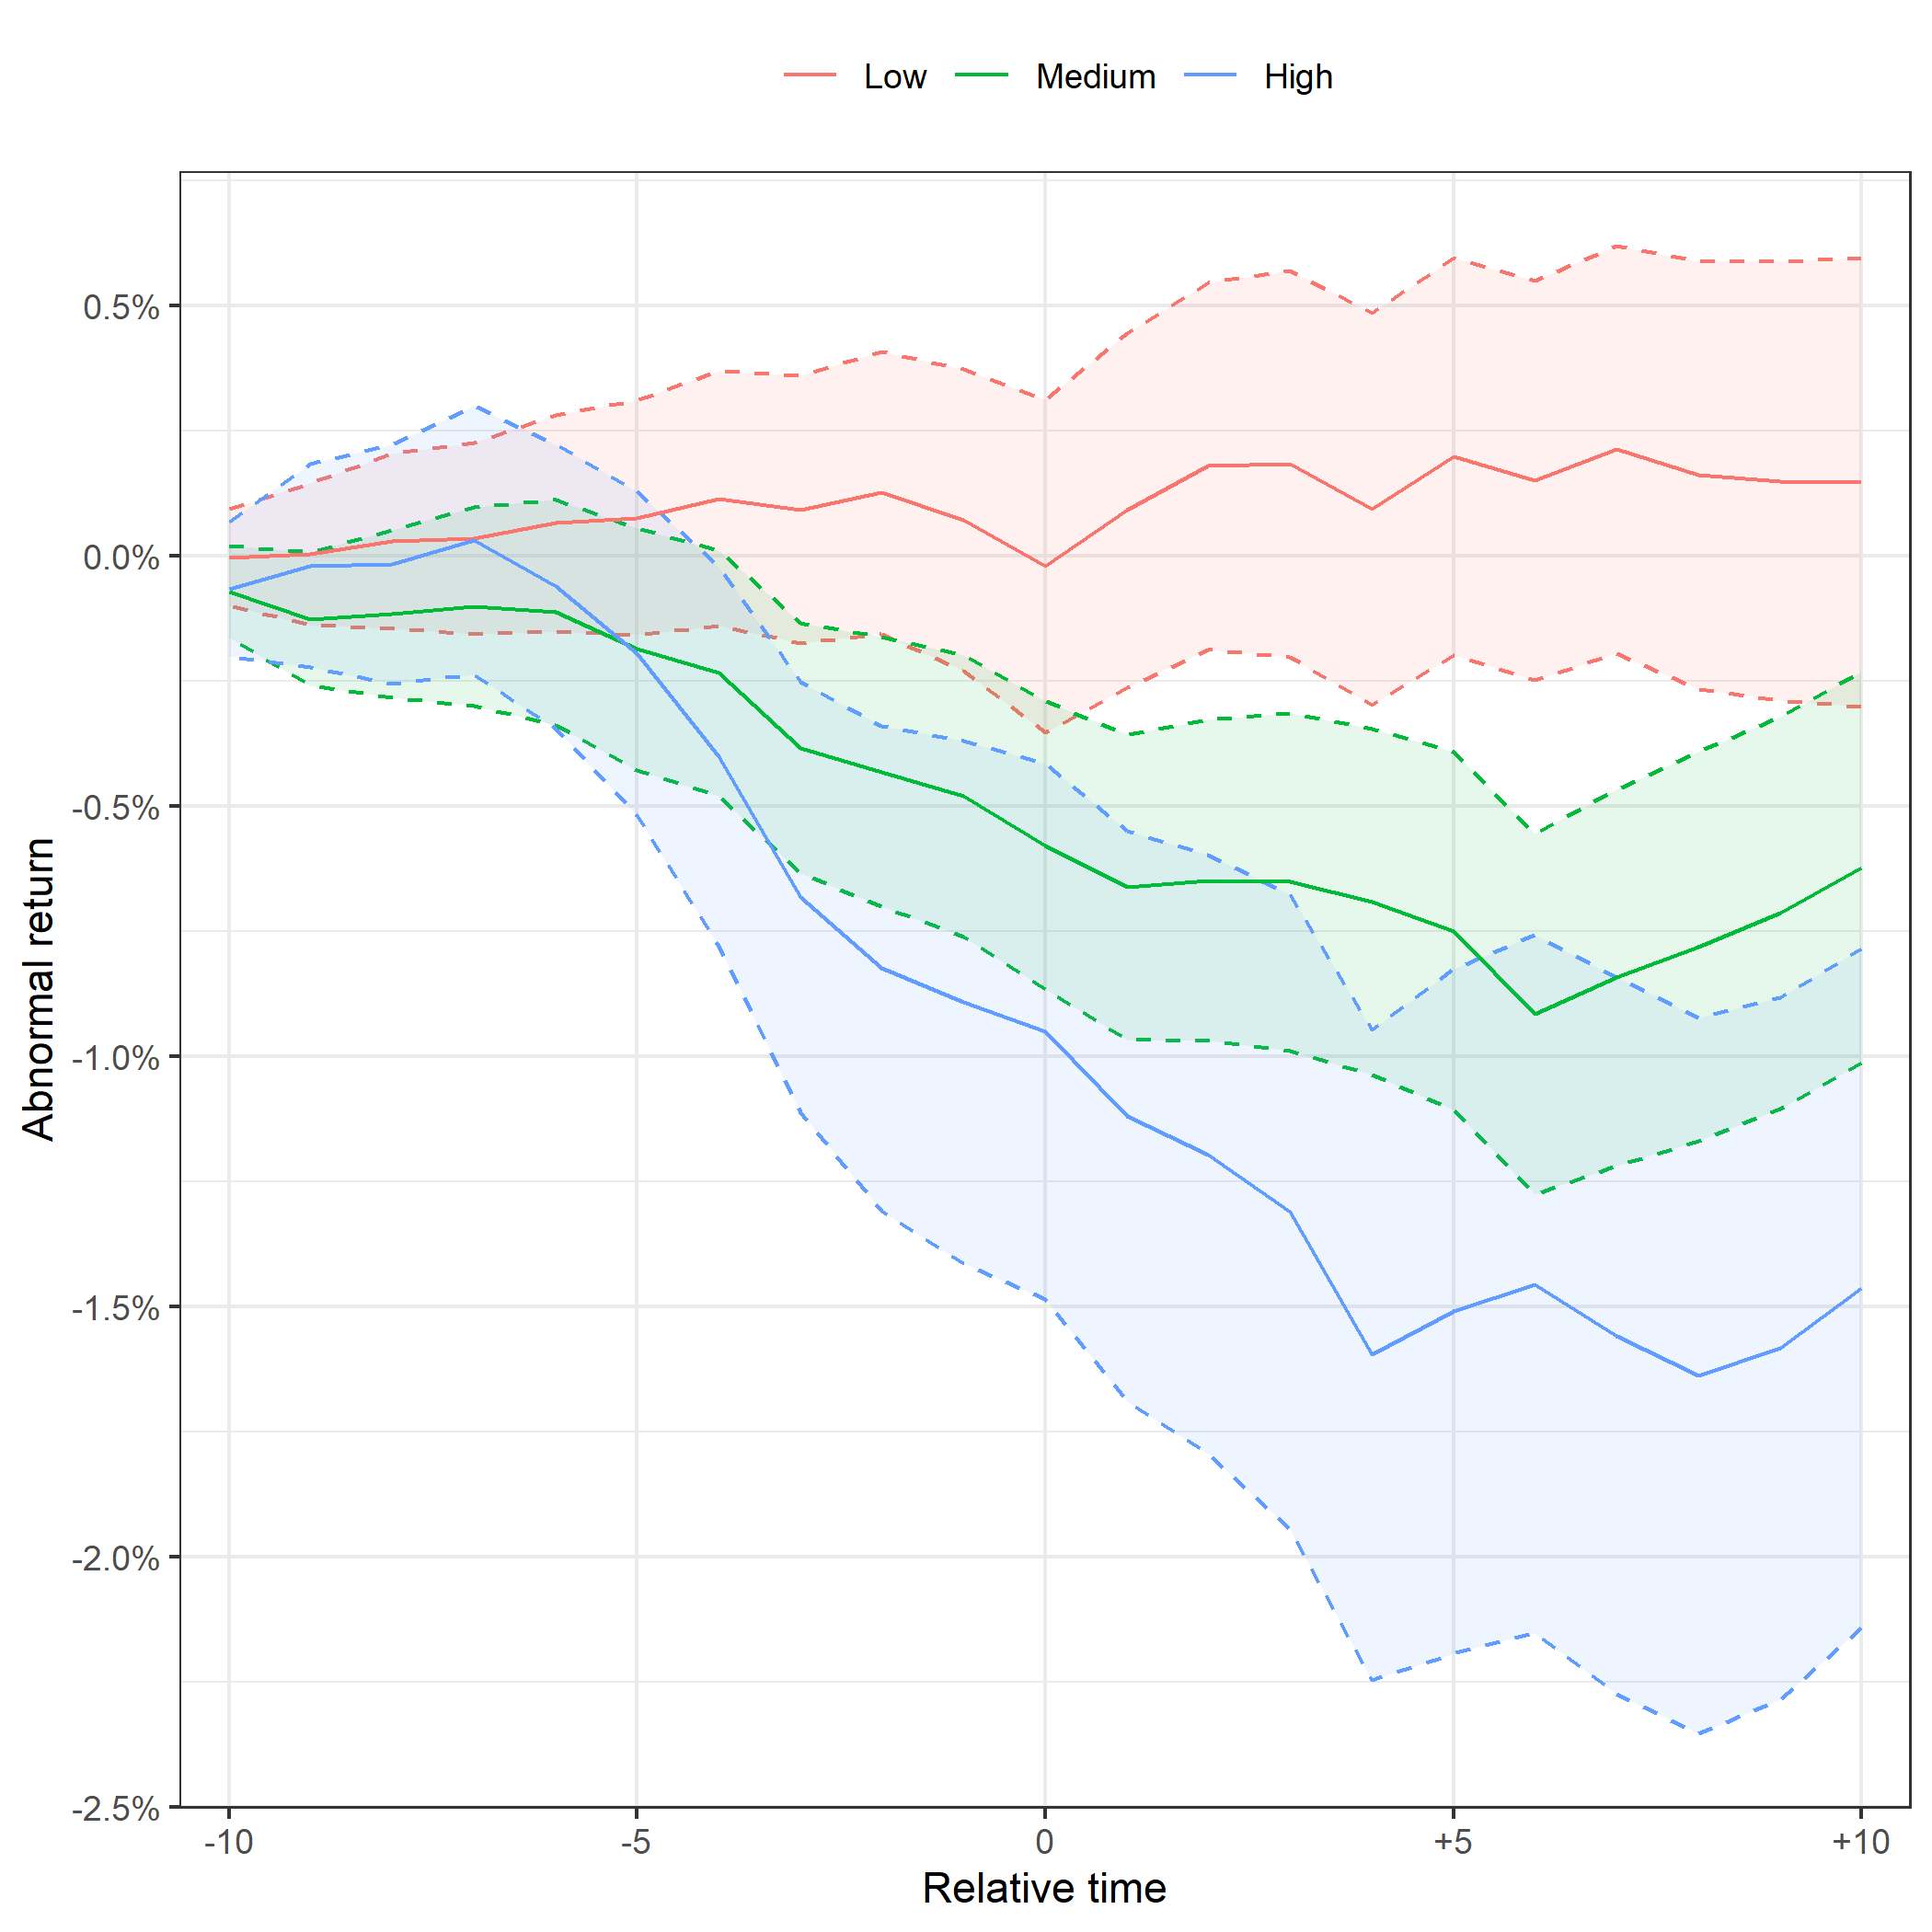
\includegraphics[width=\textwidth]{Projekt/1.Figures analysis/ST_negative_ESG_nasdaq.png}
    \label{fig:ST_neg_sensitivity_nasdaq_ESG}
     \end{minipage}
        \caption*{\footnotesize The figure illustrates the average abnormal return (AAR) and cumulative AAR (CAAR) around the event date (t = 0) of negative news. The blue lines are returns calculated from an equally weighted portfolio, while the red lines are based on market capitalization weights. 5.138 daily events }
        
        \label{fig:three graphs}
\end{figure}

Figure \ref{fig:ST_neg_sensitivity_nasdaq} illustrates that the short-term market reaction to negative news from the global sample exhibits a similar pattern to that of the European, with the majority of the decline in market value occurring prior to the events being identified. However, the reaction in Europe tend to be slightly more negative compared to global companies, with CAAR values of -0.72\% and -0.56\%, respectively. On the contrary, when partitioning on ESG risk levels as in figure \ref{fig:ST_neg_sensitivity_nasdaq_ESG}, the inferences shift around. Negative news has minimal impact on market values for global low-risk companies, with a CAAR remaining close to zero throughout the full window. Conversely, European companies experience a notable decline with an average loss of -1.65\% over the 21-day window.  Global high-risk companies suffer a substantial market value loss of approximately -1.5\%, while medium-risk firms show a reaction similar to European equities. 

The short-term impact of positive news on global companies differs slightly from that of European companies. High-risk companies, in particular, tend to receive greater, but insignificant, average rewards for positive news, while the impact on medium and low-risk companies is minimal. However, since the remaining part of the paper will focus mostly on negative news, I will do the same here. Thus, the AAR and CAAR for all firms and split on ESG risk for positive events are available in tables \ref{fig:ST_pos_sensitivity_nasdaq} and \ref{fig:ST_pos_sensitivity_nasdaq_ESG} in appendix \ref{app: sensitivity}.

\setlength{\tabcolsep}{15pt}
\begin{table}[H]
\small
\centering
\caption{Fama-French five-factor model alpha from NASDAQ negative news split on ESG risk} 
\begin{tabular}{ccccccc}
\hline \hline \\ 
 &     & Overall &    Low  &  Medium  &  High &  \\    \cline{3-6} 
& &  \multicolumn{4}{c}{ T = 1} & \\ \cline{2-6}
& Alpha  & -0.26 & -0.40  & -0.29  & -0.11 &  \\ 
& t-value   & -1.06 & -1.03 & -0.76  & -0.18 &  \\
& &  \multicolumn{4}{c}{ T = 4} & \\ \cline{2-6}
& Alpha & $-0.34^{*}$  & -0.26  & $-0.45^{**}$  &  $-0.58^{*}$ & \\
& t-value &   -1.92 & -1.14 & -2.16  & -1.69 & \\
& &  \multicolumn{4}{c}{ T = 8} & \\ \cline{2-6}
& Alpha & $-0.29^{**}$ & -0.24  & -0.24  & $-0.51$ &  \\
& t-value & -2.14 & -1.19  & -1.53 & -1.50 &  \\
& &  \multicolumn{4}{c}{ T = 12} & \\ \cline{2-6}
& Alpha  & $-0.35^{***}$ & -0.29  & $-0.36^{**}$  & $-0.46$ &  \\
& t-value & -3.28 & -1.56  & -2.51 & -1.40 &  \\
\hline \hline
 \multicolumn{7}{l}{ \footnotesize $^* \; p\; <\; 0.1$, $ ^{**} \; p\; <\; 0.05$, $ ^{***} \; p\; <\; 0.01$  } \\
 \multicolumn{7}{p{11.5cm}}{ \footnotesize Alpha is the WLS-regression intercept (in \%) of the Fama-French 5-factor model, displayed along with the corresponding White heteroskedasticity-robust t-value. N is the average amount of firms included in the portfolio each month, and T is the portfolio holding period. The threshold for event firms to be included in the portfolio is either 1,2 or 3 "SD" (standard deviations) larger than the mean. N = 3.945 } \\ 
 \hline
\end{tabular}
\label{tab: FF5_neg_nasdaq}
\end{table}

On a general level, the long-term alphas are in line with the outcome from the short-term. The first column in table \ref{tab: FF5_neg_nasdaq} illustrate that global firms face a persistent penalty lasting beyond 12 months. Portfolios with holding periods of four, eight, and 12 months exhibit negative and statistically significant alpha values, on at least a 10\% level,  ranging from -0.29\% to -0.35\%. 

However, a partition on ESG risk indicates that the inferences from the short-term analysis does not hold over longer horizons for all risk types. The high-risk portfolio, which suffered a short term loss of -1.5\%, generates an alpha close to zero, at -0.11\% when applying a one month holding period. Increasing the holding period to four months or longer leads to more negative alphas at a stable level around -0.5\%, more in line with the expectations from the short term. The dramatic development is unintuitive, but may be an indication of a possible initial overreaction, but a consistent long-term market penalty. As the low-risk portfolio doesn't generate significant alpha at any point, it seems the intuition from the short term results holds. The firms in the medium-risk portfolio is penalized slightly over a longer horizons. However, no general conclusions can be made, since the significance of the alpha values fluctuate with holding periods. 

In summary, the initial parts of the sensitivity analysis, which has its focus on European stocks, reveal that the short-term models consistently demonstrate a negative shareholder reaction to adverse events, and the magnitude of the reactions remain relatively stable. Moreover, the altered long-term results has two implications. First, as the sign of the alphas remain negative, the negative reactions to adverse events is robust. Second, tightening the event threshold leads to unstable but negative investor reactions. In addition, in Europe and the rest of the world, corporate negative SDG news are penalized by investors. However, investors are in disagreement on how to penalize companies when accounting for ESG risk. In the following chapter I will collect all of the results and, to the best of my ability, provide intuition to the findings along with perspectives from related research. 